\section{Results and discussion}

% results from my pipelines automatic sleep staging
% no ground truth but multirater cooperation. hypnogram comparison with patricia, metrics, conf matrices
% hypnogram comparison with GT for sleepEDFdatabse



% only 2 recordings
In total, only 2 overnight EEG sleep recordings (from 2 different healthy adult makes) were used in the pipeline during the course of this project. They were produced in the European Data Format (.edf). The recordings were taken from a 27 channel EEG setup used interally for clinical trials. 
However, as was described, the pipeline is prepared to receive more data, and obtaining the predictions for them is streamlined.
\\
% redundant to report on all
Reporting on all sleep recordings is, therefore, slightly redundant, as the goal was not to obtain good results for one patient, but streamlining obtaining those results for a cohort of subjects fast and efficiently. With this, only the results for one of the subjects will be shown on most plots, to be used as an ilustrative example of the pipeline's functioning and output formats. 


\subsection{Sleep staging results}
% hypnogram results
From the \texttt{visualize\_hypnogram} script, the hypnogram  (Fig.\ref{fig:hypnograms_30_120}) and prediction probabilities plot (Fig.\ref{fig:hypnogram_probs_30}) are produced based on the predictions.pkl files for each subject, which are the output of the pipeline in \cite{Alexander2020}.

\vspace{-0.2cm}

% hypnograms with 2 windowsizes
\begin{figure}[H]
    \centering
    \begin{subfigure}[b]{0.46\textwidth}
        \centering
        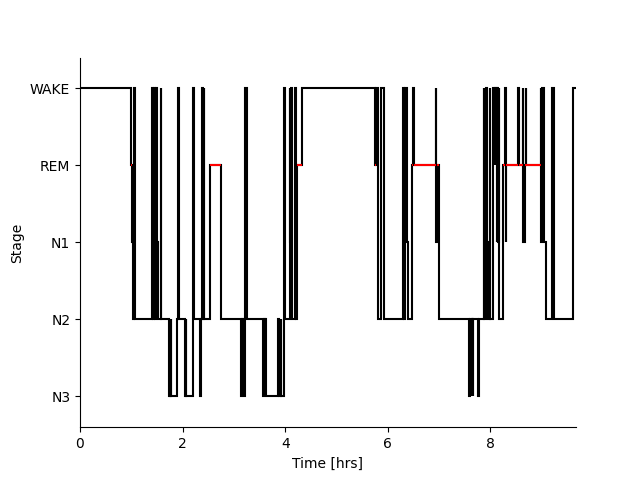
\includegraphics[width=\textwidth]{Images/marcus_hypnogram_30.png}
        \caption{Hypnogram with window of 30 epochs}
        \label{fig:hypnogram_30}
    \end{subfigure}
    \hfill
    \begin{subfigure}[b]{0.46\textwidth}
        \centering
        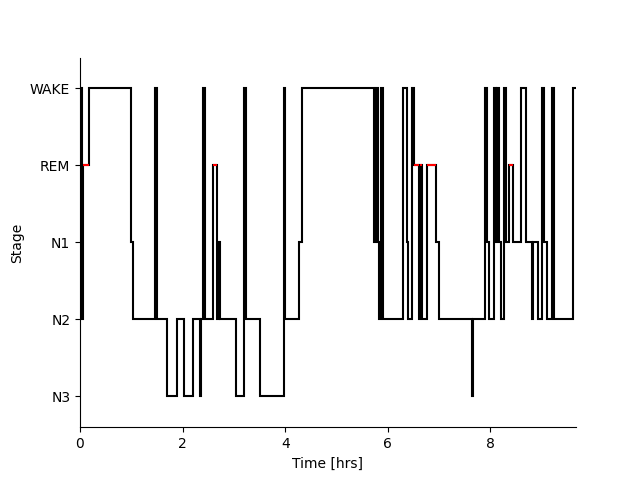
\includegraphics[width=\textwidth]{Images/marcus_hypnogram_120.png}
        \caption{Hypnogram with window of 120 epochs}
        \label{fig:hypnogram_120}
    \end{subfigure}
    \vspace{-0.1cm}
    \caption{Predicted hypnograms for the same data, for 2 window sizes}
    \label{fig:hypnograms_30_120}
\end{figure}


% probs hypnogram
\vspace{-1cm}
\begin{figure}[H]
    \centering
    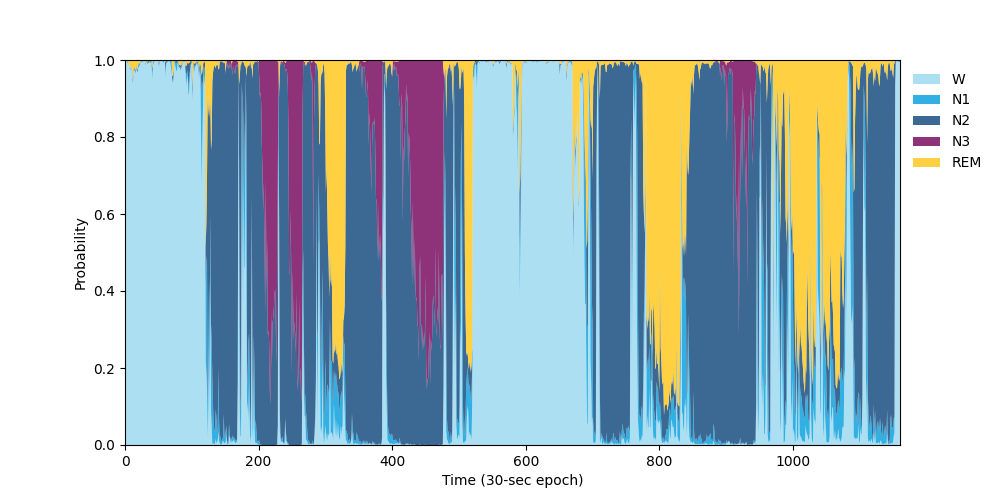
\includegraphics[width=0.7\linewidth]{Images/marcus_hypnogram_probs_30.png}
    \caption{Probabilities for each sleep stage for each epoch}
    \label{fig:hypnogram_probs_30}
\end{figure}

% explain the 2 windowsizes
The results from Fig.\ref{fig:hypnogram_30} and Fig.\ref{fig:hypnogram_120} were obtained by running the \texttt{display\_hypnogram} twice, with different window sizes. A initial index of 18000 was also used, as the recording had a few hours where the subject was still awake. As expected, the result with a bigger window (2 minutes) is smoother but loses a lot of time resolution. Namely, the amount of predicted REM sleep is almost halved with a bigger window. This stage of the sleep cycle can sometimes be very short ($\sim$5 minutes), and the bigger window might have a harder time picking it up.

% explain the probas plot
On the other hand, Fig.\ref{fig:hypnogram_probs_30} shows the predictions' confidence of each sleep stage for each 30 seconds epoch. In essence, each point in the hypnogram in Fig.\ref{fig:hypnogram_30} is the sleep stage with the highest probability for that epoch from the predicted hypnogram probabilities (Fig.\ref{fig:hypnogram_probs_30}).





\subsection{Multi-rater comparison}
% explian where the data came from
For the multi-rater comparison of results from different pipelines, it was imperative that the predictons from each were in the same format. Because the results from the pipeline used by my collegue (\cite{2021yasa,belonosov2023sleepeegpy}) automatically exported the predictions in the txt format mentioned (with the prediction for each epoch in each line), running the \texttt{predictions\_to\_txt} on the predictions from this pipeline would ensure coherence. Like for visualizing the hypnogram, the \texttt{predictions\_to\_txt} script was run twice with 2 different values for the evaluation window: 30 and 60 seconds. After placing these 2 txt files (\texttt{subj-1\_win-30.txt} and \texttt{subj-1\_win-60.txt}) as well as the one produced from the other pipeline (\texttt{model2\_subj-1\_win-30.txt}), all 3 obtained from the same sleep EEG data, in the same folder, running the \texttt{hypnogram\_comparison} script produced the plots below. It is important to mention that, as the first two files were produced from the same predictions but with different sizes of prediction windows, the results between these two were expected to be quite simillar, and were included side to side as a form of control.



% TALK ABOUT THE SUPERIMPOSED AND CM
In Fig.\ref{fig:multirater_hypnogram}, the superimposed predicted hypnogram for each of the 3 models is shown. Together with the confusion matrix of preditions between \texttt{model2\_subj-1\_win-30} and \texttt{subj-1\_win-30}, we show that these two models agree on most pairs of predictions, most notably in the wake and REM stages. Cruacially, there seems to be less agreement in the light and deep sleep, with model 1 \cite{Alexander2020} predicting more light sleep (N1) and model 2 \cite{2021yasa} predicting more deep sleep, in general.

% number of raters
Due to the lack of real annotated data, the number of raters that agree on the predicted sleep stage for a certain time stamp is a good proxi for the confidence on the prediction of the ensemble. And, if all raters, i.e. all automatic sleep staging algorithms used, agree on a certain prediction, we could, to a certain degree of confidence, assume that as the true predicted label for that time stamp. Fig.\ref{fig:number_of_agreers} shows that on 85\% of the time, all 3 predictions agree, which is already a good sign that the predictions are not far from the truth.


% multirater hypnogram
\begin{figure}[H]
    \centering
    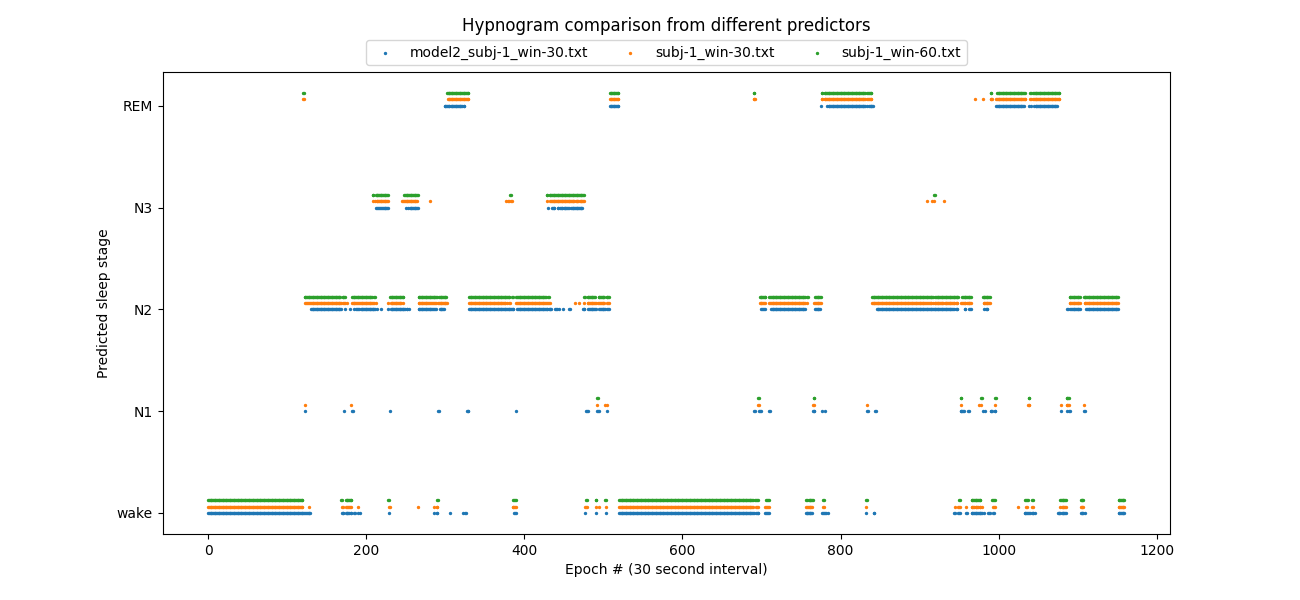
\includegraphics[width=0.99\linewidth]{Images/comparisson1_hypnogramComparison.png}
    \vspace{-0.8em}
    \caption{Multi-rater hypnogram predictions}
    \label{fig:multirater_hypnogram}
\end{figure}



% CM for all predictions between 2 models
\vspace{-0.9cm}
\begin{figure}[H]
    \centering
    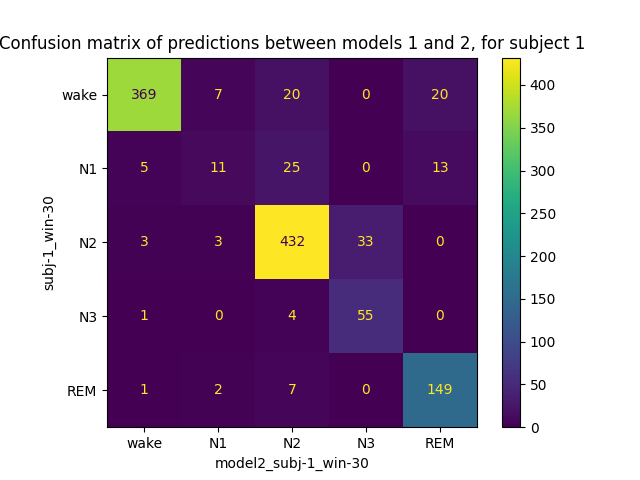
\includegraphics[width=0.55\linewidth]{Images/comparisson1_predictionsCM.png}
    \vspace{-0.8em}
    %\caption{Probability of 1, 2 or 3 of the predictions agreeing for any time stamp}
    \caption{Confusion matrix for all epoch predictions between \texttt{model2\_subj-1\_win-30} and \texttt{subj-1\_win-30} }
    \label{fig:CM_between_2_raters}
\end{figure}



% number of agreers 
\vspace{-1cm}
\begin{figure}[H]
    \centering
    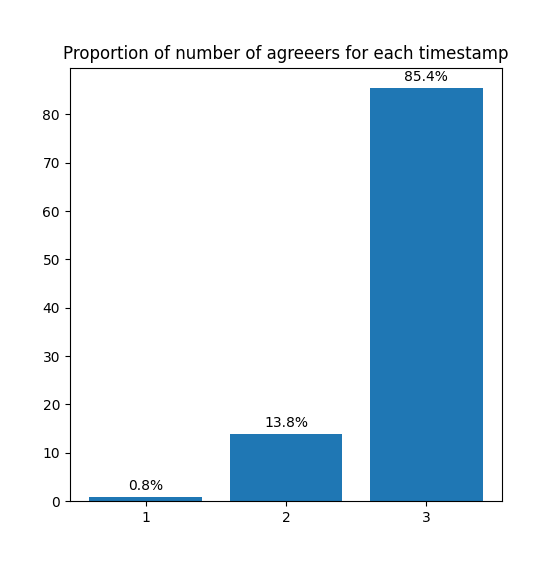
\includegraphics[width=0.4\linewidth]{Images/comparisson1_numAgreers.png}
    \vspace{-1em}
    %\caption{Probability of 1, 2 or 3 of the predictions agreeing for any time stamp}
    \caption{Percentage of time stamps where none, 2 or all 3 prediction models agree}
    \label{fig:number_of_agreers}
\end{figure}



% agreements and kappa score
\begin{figure}[H]
    \centering
    \begin{subfigure}[b]{0.48\textwidth}
        \centering
        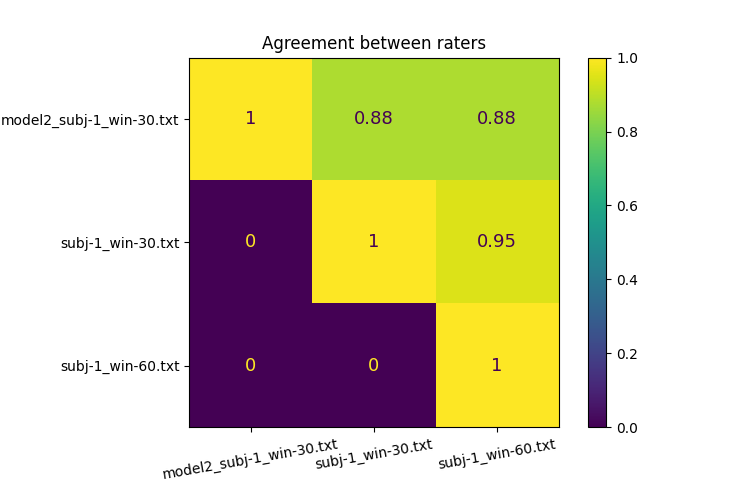
\includegraphics[width=\textwidth]{Images/comparisson1_accuracyCM.png}
        \caption{Agreement between each pair of raters}
        \label{fig:multirater_agreementCM}
    \end{subfigure}
    %\hfill
    \hspace{-0.5cm}
    \begin{subfigure}[b]{0.48\textwidth}
        \centering
        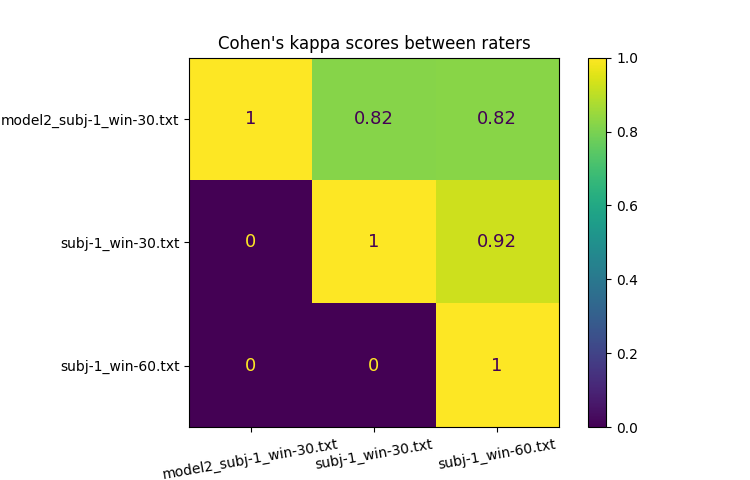
\includegraphics[width=\textwidth]{Images/comparisson1_kappaCM.png}
        \caption{Kappa score between each pair of raters}
        \label{fig:multirater_kappaCM}
    \end{subfigure}
    \caption{Agreement and Kappa scores between each pair of raters}
    \label{fig:multirater_CMs}
\end{figure}


% CM of agreement and of kappa - EXPLANATION
Fig.\ref{fig:multirater_agreementCM} shows the percentage of agreement between each pair of models. Likewise, Fig.\ref{fig:multirater_kappaCM}, shows the Kappa score between each pair of model predictions. 
The diagonal of the matrix is, by definition, just ones, and the lower triangular matrix was displayed as zeros to avoid confusion, but the matrices are essencially simetrical because both agreement and Kappa score are invariant to changing the order of the pair of models.

% CM of agreement and of kappa - IN DEPTH
As expected, the agreement and Kappa score are almost 1 between \texttt{subj-1\_win-30} and \texttt{subj-1\_win-60} (0.95 and 0.92 for agreement and kappa, respectively). 
Both metrics were the same between any of the predictions with different window sizes from model 1 and the predictions from model 2 (0.88 agreement and 0.82 kappa score). 
With all this, the multi-rater ensemble-like setup demonstrated quite good levels of agreement between multiple models, and proved to be a satisfactory automatic sleep staging algorithm.



% RESULTS FOR OTHER PATIENT TESTED
\subsection*{Results for subject 2} %\#
The results from performing the same analysis on the second subject were not displayed, but some analysis can still be done. The agreement and kappa score between the pipeline used here and the pipeline used by my collegue were of 0.77 and 0.64, which is slightly lower than for the first subject. The 2 raters had quite good agreement with N2 and awake states, but performed poorly on the other sleep stages. Fig.\ref{fig:Appendix_subj2_multirater_hypnogram} in the appendix shows the hypnogram each of the 2 models predicted, superimposed.




\subsection{Validation with ground truth dataset}
% why do this
Finally, a small validation study on a simple EEG sleep dataset with annotated hypnograms was done. This exercise was do to try to validate the model and pipeline in a labeled dataset consisting in sleep data more similar to the EEG setup being used in Optoceutics' research. In other words, to assess if this model performed well enough against EEG only annotated data.

% only one datapoint and how to run
For this analysis, due to lack of time, only the first entry in the sleep EDF database \cite{kemp2018sleepEDFwebsite,2000sleepEDForiginal} was used. The steps of the pipeline were run in sequence as prescribed, treating the new data as a new cohort. In the end, instead of comparing the predicted hypnogram from 2 different raters, the results from this pipeline were compared to the labeled hypnogram. 

% results
The small validation study provided satisfactory results, with accuracy of 78\% but a Cohen's kappa score of only 0.55. The side by side hypnogram comparison as well as the confusion matrix between the predicted and ground truth labeled data can be found in the appendix (Fig.\ref{fig:Appendix_GT_hypnogram} and Fig.\ref{fig:Appendix_GT_CM}). The prediction model tended to overpredict the REM stage when the patient should have stil been awake, but the N2 and especially N3 were predicted relatively accurately. Another relevant finding is that, while the prediction model oscilates between different predictions in sequential 30s epochs, the ground truth is far more smooth and continuous.

